\begin{figure}
    \centering
    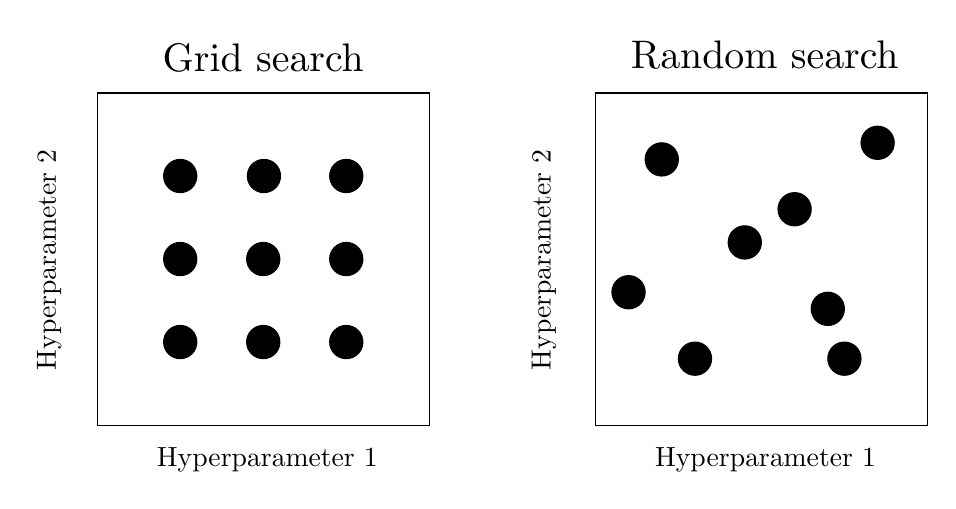
\begin{tikzpicture}[x=0.6pt,y=0.6pt,yscale=-1,xscale=1]
        %Shape: Rectangle [id:dp7765345595299928] 
        \draw   (40,40) -- (240,40) -- (240,240) -- (40,240) -- cycle ;
        %Shape: Rectangle [id:dp8266179045308344] 
        \draw   (340,40) -- (540,40) -- (540,240) -- (340,240) -- cycle ;
        %Shape: Circle [id:dp10989848309136652] 
        \draw  [fill={rgb, 255:red, 0; green, 0; blue, 0 }  ,fill opacity=1 ] (80,90) .. controls (80,84.48) and (84.48,80) .. (90,80) .. controls (95.52,80) and (100,84.48) .. (100,90) .. controls (100,95.52) and (95.52,100) .. (90,100) .. controls (84.48,100) and (80,95.52) .. (80,90) -- cycle ;
        %Shape: Circle [id:dp25798568532386523] 
        \draw  [fill={rgb, 255:red, 0; green, 0; blue, 0 }  ,fill opacity=1 ] (130.4,90) .. controls (130.4,84.48) and (134.88,80) .. (140.4,80) .. controls (145.92,80) and (150.4,84.48) .. (150.4,90) .. controls (150.4,95.52) and (145.92,100) .. (140.4,100) .. controls (134.88,100) and (130.4,95.52) .. (130.4,90) -- cycle ;
        %Shape: Circle [id:dp21802627978178712] 
        \draw  [fill={rgb, 255:red, 0; green, 0; blue, 0 }  ,fill opacity=1 ] (180,90) .. controls (180,84.48) and (184.48,80) .. (190,80) .. controls (195.52,80) and (200,84.48) .. (200,90) .. controls (200,95.52) and (195.52,100) .. (190,100) .. controls (184.48,100) and (180,95.52) .. (180,90) -- cycle ;
        %Shape: Circle [id:dp29856163256776613] 
        \draw  [fill={rgb, 255:red, 0; green, 0; blue, 0 }  ,fill opacity=1 ] (80,140) .. controls (80,134.48) and (84.48,130) .. (90,130) .. controls (95.52,130) and (100,134.48) .. (100,140) .. controls (100,145.52) and (95.52,150) .. (90,150) .. controls (84.48,150) and (80,145.52) .. (80,140) -- cycle ;
        %Shape: Circle [id:dp29841099273644034] 
        \draw  [fill={rgb, 255:red, 0; green, 0; blue, 0 }  ,fill opacity=1 ] (130,140) .. controls (130,134.48) and (134.48,130) .. (140,130) .. controls (145.52,130) and (150,134.48) .. (150,140) .. controls (150,145.52) and (145.52,150) .. (140,150) .. controls (134.48,150) and (130,145.52) .. (130,140) -- cycle ;
        %Shape: Circle [id:dp49228249173727456] 
        \draw  [fill={rgb, 255:red, 0; green, 0; blue, 0 }  ,fill opacity=1 ] (180,140) .. controls (180,134.48) and (184.48,130) .. (190,130) .. controls (195.52,130) and (200,134.48) .. (200,140) .. controls (200,145.52) and (195.52,150) .. (190,150) .. controls (184.48,150) and (180,145.52) .. (180,140) -- cycle ;
        %Shape: Circle [id:dp38157661859427416] 
        \draw  [fill={rgb, 255:red, 0; green, 0; blue, 0 }  ,fill opacity=1 ] (80,190) .. controls (80,184.48) and (84.48,180) .. (90,180) .. controls (95.52,180) and (100,184.48) .. (100,190) .. controls (100,195.52) and (95.52,200) .. (90,200) .. controls (84.48,200) and (80,195.52) .. (80,190) -- cycle ;
        %Shape: Circle [id:dp13924586669074634] 
        \draw  [fill={rgb, 255:red, 0; green, 0; blue, 0 }  ,fill opacity=1 ] (130,190) .. controls (130,184.48) and (134.48,180) .. (140,180) .. controls (145.52,180) and (150,184.48) .. (150,190) .. controls (150,195.52) and (145.52,200) .. (140,200) .. controls (134.48,200) and (130,195.52) .. (130,190) -- cycle ;
        %Shape: Circle [id:dp30928749690617674] 
        \draw  [fill={rgb, 255:red, 0; green, 0; blue, 0 }  ,fill opacity=1 ] (180,190) .. controls (180,184.48) and (184.48,180) .. (190,180) .. controls (195.52,180) and (200,184.48) .. (200,190) .. controls (200,195.52) and (195.52,200) .. (190,200) .. controls (184.48,200) and (180,195.52) .. (180,190) -- cycle ;
        %Shape: Circle [id:dp4482564100459898] 
        \draw  [fill={rgb, 255:red, 0; green, 0; blue, 0 }  ,fill opacity=1 ] (370,80) .. controls (370,74.48) and (374.48,70) .. (380,70) .. controls (385.52,70) and (390,74.48) .. (390,80) .. controls (390,85.52) and (385.52,90) .. (380,90) .. controls (374.48,90) and (370,85.52) .. (370,80) -- cycle ;
        %Shape: Circle [id:dp07124098077781627] 
        \draw  [fill={rgb, 255:red, 0; green, 0; blue, 0 }  ,fill opacity=1 ] (420,130) .. controls (420,124.48) and (424.48,120) .. (430,120) .. controls (435.52,120) and (440,124.48) .. (440,130) .. controls (440,135.52) and (435.52,140) .. (430,140) .. controls (424.48,140) and (420,135.52) .. (420,130) -- cycle ;
        %Shape: Circle [id:dp41745813324763004] 
        \draw  [fill={rgb, 255:red, 0; green, 0; blue, 0 }  ,fill opacity=1 ] (390,200) .. controls (390,194.48) and (394.48,190) .. (400,190) .. controls (405.52,190) and (410,194.48) .. (410,200) .. controls (410,205.52) and (405.52,210) .. (400,210) .. controls (394.48,210) and (390,205.52) .. (390,200) -- cycle ;
        %Shape: Circle [id:dp5867108869326927] 
        \draw  [fill={rgb, 255:red, 0; green, 0; blue, 0 }  ,fill opacity=1 ] (450,110) .. controls (450,104.48) and (454.48,100) .. (460,100) .. controls (465.52,100) and (470,104.48) .. (470,110) .. controls (470,115.52) and (465.52,120) .. (460,120) .. controls (454.48,120) and (450,115.52) .. (450,110) -- cycle ;
        %Shape: Circle [id:dp562496351098612] 
        \draw  [fill={rgb, 255:red, 0; green, 0; blue, 0 }  ,fill opacity=1 ] (480,200) .. controls (480,194.48) and (484.48,190) .. (490,190) .. controls (495.52,190) and (500,194.48) .. (500,200) .. controls (500,205.52) and (495.52,210) .. (490,210) .. controls (484.48,210) and (480,205.52) .. (480,200) -- cycle ;
        %Shape: Circle [id:dp7209986165291683] 
        \draw  [fill={rgb, 255:red, 0; green, 0; blue, 0 }  ,fill opacity=1 ] (470,170) .. controls (470,164.48) and (474.48,160) .. (480,160) .. controls (485.52,160) and (490,164.48) .. (490,170) .. controls (490,175.52) and (485.52,180) .. (480,180) .. controls (474.48,180) and (470,175.52) .. (470,170) -- cycle ;
        %Shape: Circle [id:dp586705666058086] 
        \draw  [fill={rgb, 255:red, 0; green, 0; blue, 0 }  ,fill opacity=1 ] (500,70) .. controls (500,64.48) and (504.48,60) .. (510,60) .. controls (515.52,60) and (520,64.48) .. (520,70) .. controls (520,75.52) and (515.52,80) .. (510,80) .. controls (504.48,80) and (500,75.52) .. (500,70) -- cycle ;
        %Shape: Circle [id:dp7017198962451507] 
        \draw  [fill={rgb, 255:red, 0; green, 0; blue, 0 }  ,fill opacity=1 ] (350,160) .. controls (350,154.48) and (354.48,150) .. (360,150) .. controls (365.52,150) and (370,154.48) .. (370,160) .. controls (370,165.52) and (365.52,170) .. (360,170) .. controls (354.48,170) and (350,165.52) .. (350,160) -- cycle ;
        
        % Text Node
        \draw (142.5,261) node  [align=left] {Hyperparameter 1};
        % Text Node
        \draw (442.5,261) node  [align=left] {Hyperparameter 1};
        % Text Node
        \draw (11,140.5) node [rotate=-270] [align=left] {Hyperparameter 2};
        % Text Node
        \draw (309,140.5) node [rotate=-270] [align=left] {Hyperparameter 2};
        % Text Node
        \draw (140,19) node [scale=1.44] [align=left] {Grid search};
        % Text Node
        \draw (442,17) node [scale=1.44] [align=left] {Random search};
    \end{tikzpicture}

    \caption{Grid and random search of nine trials. With grid search, nine trials only test three distinct values for each hyperparameter. On the other hand, with random search nien different values are explored for each hyperparameter. If one of these hyperparameters is much more important than the other (as is often the case) then random search is more likely to find promising regions of the space.}
    \label{grid_vs_random}
\end{figure}    